\chapter{Impostazione del laboratorio}\label{imp_laboratorio}
In questo capitolo verranno analizzati tutti gli strumenti utilizzati per l'implementazione dell'ambiente di simulazione e il modo in cui esso viene avviato. In particolare verranno presentati: gli strumenti per la realizzazione del laboratorio, gli strumenti utilizzati per il monitoraggio della rete dove opera il laboratorio e il modo in cui viene effettivamente implementata la botnet Mirai.
\section{Strumenti di simulazione}\label{strumenti_di_simulazione}
Al fine di riprodurre il comportamento della botnet Mirai, quanto più fedelmente possibile, è stato implementato un laboratorio completamente isolato. 
La configurazione del laboratorio, di seguito descritta, si basa su un progetto disponibile pubblicamente su GitHub\footnote{\url{https://github.com/luiss07/mirai}}, il quale riadatta il codice sorgente della prima versione di Mirai per riprodurne il comportamento in un ambiente locale tramite l'ausilio di Docker\footnote{\url{https://www.docker.com/}}. La prima differenza visibile, rispetto alla versione originale di Mirai, è la mancanza del report server e del loader server, nello specifico il report server è stato eliminato mentre il loader server è stato integrato all'interno del CNC server. Un'altra parte che ha subito cambiamenti rispetto all'originale è quella relativa alla scansione della rete da parte dei bot alla ricerca di nuovi dispositivi infettabili. Infatti mentre il codice originale, relativo alla scansione, era scritto in linguaggio C in questo progetto è stato scritto in linguaggio Python. Questa modifica semplifica l’implementazione nel contesto di un laboratorio locale, poiché gli indirizzi IP da analizzare non vengono individuati tramite una scansione casuale della rete, ma sono prelevati da un array definito all’interno dello script Python. In questo modo è possibile controllare con precisione i dispositivi da prendere di mira per la scansione. Infine, poiché nel laboratorio i container vulnerabili utilizzano tutti la stessa architettura, non è più necessario generare molteplici eseguibili tramite i 10 cross-compiler previsti nella versione originale di Mirai. Questo semplifica ulteriormente il processo di infezione e lo rende più adatto a un ambiente di test controllato.
L’idea alla base della configurazione scelta è quella di installare una macchina virtuale e isolarla completamente dall’host principale, per motivi di sicurezza, tramite una rete isolata che ne impedisce la comunicazione con quest'ultimo. Una volta predisposto l’ambiente isolato, la macchina viene dotata di Docker e utilizzata per avviare l’intero laboratorio. Nel nostro caso la macchina virtuale utilizzata per installare l'ambiente di analisi è Kali Linux\footnote{\url{https://www.kali.org/}}, tale scelta è motivata dal fatto che questa distribuzione di Debian dispone sin da subito di una grande vastità di strumenti di sicurezza informatica, analisi di rete e penetration testing.  Nel nostro caso specifico alcuni di questi strumenti hanno permesso di comprendere al meglio il funzionamento generale della botnet. 
Come già detto in precedenza la macchina virtuale deve essere dotata di Docker che è una piattaforma per la creazione e la gestione di applicazioni in \emph{container}. Un container comprende sia l'applicazione che le librerie necessarie per il suo funzionamento isolandolo dal sistema operativo sottostante. I vantaggi sono molteplici:
\begin{itemize}
    \item \textbf{Maggiore efficienza}: i container sono leggeri e richiedono meno risorse rispetto l'esecuzione di molteplici applicazioni;
    \item \textbf{Portabilità}: una configurazione può essere facilmente replicata in un altro dispositivo;
    \item \textbf{Isolamento}: i container sono isolati dal sistema operativo sottostante offrendo maggiore sicurezza;
    \item \textbf{Scalabilità}: i container possono essere scalati per andare a soddisfare le esigenze dell'applicazione.
\end{itemize}

Un container viene eseguito a partire da un'immagine preesistente che può essere personalizzata per essere adattata alle proprie esigenze. Tipicamente questa personalizzazione avviene per mezzo di un \emph{Dockerfile}. Docker permette anche l'avvio rapido di uno o più container tramite l'esecuzione di un file in formato \texttt{.yml}. Nel nostro caso specifico Docker è stato usato per andare a riprodurre, quanto più fedelmente possibile, l'ambiente operativo dei nodi della botnet. In particolare i container sono stati configurati per comportarsi come sistemi operativi completi al fine di emulare: server CNC, bot attaccanti, bot-scanner e server vittima. L'esigenza di utilizzare Docker nasce dal fatto che lo stesso ambiente, riprodotto tramite l'utilizzo di macchine virtuali, sarebbe stato molto più costoso a livello di risorse. La Figura~\ref{architettura_laboratorio} descrive la topologia del laboratorio: Kali Linux, attraverso gli strumenti di monitoraggio, supervisiona l'intera infrastruttura, intercettando le comunicazioni all'interno della rete Docker bridge che permette la comunicazione alle varie componenti della botnet.
\begin{figure}[H]
    \centering
    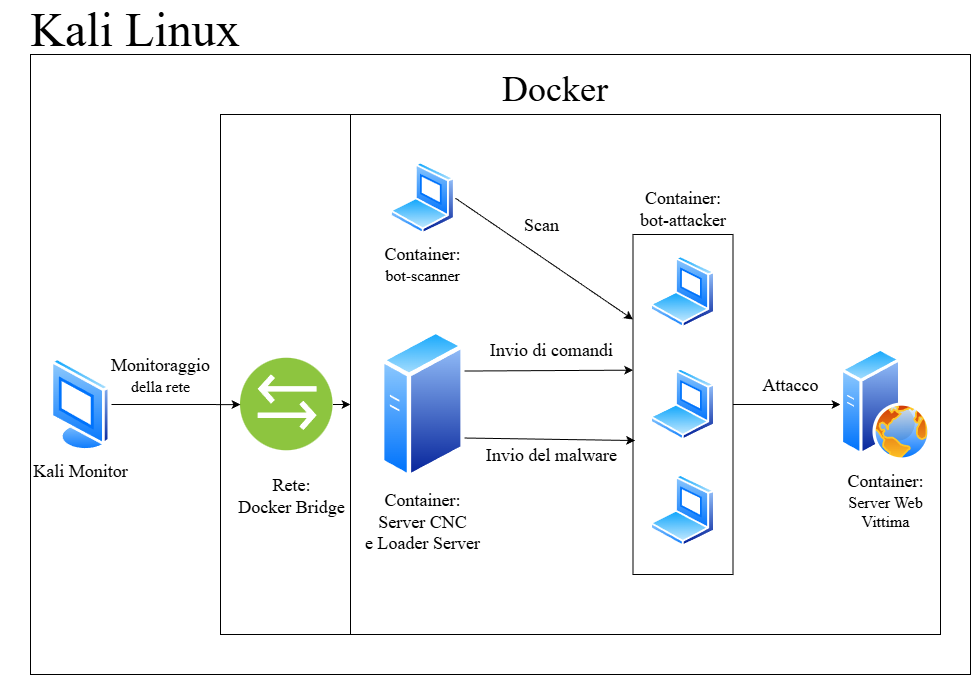
\includegraphics[width=0.75\linewidth]{tesi_stile/img/architettura_laboratorio.drawio.png}
    \caption{Architettura del laboratorio.}
    \label{architettura_laboratorio}
\end{figure}
\section{Tool di monitoraggio e analisi}\label{tool_monitoraggio}
Per andare ad analizzare il comportamento della botnet e delle sue componenti sono stati utilizzati questi strumenti nei seguenti modi:
\begin{itemize}
    \item\ \textbf{Glances}\footnote{\url{https://nicolargo.github.io/glances/}}: Glances è un software open-source che permette il monitoraggio delle risorse di un sistema. Consente un controllo in tempo reale del processore, della rete, della memoria e del disco, inoltre permette anche di visionare i processi in esecuzione. Questo strumento può essere usato tramite il terminale oppure tramite interfaccia web. Glances, nel nostro caso specifico, è stato usato per visionare come il server risponde all'arrivo massivo di pacchetti da parte dei bot, al fine di valutarne l'impatto sulle risorse del sistema;
    \item \textbf{Wireshark}\footnote{\url{https://www.wireshark.org/}}: utilizzato per andare ad analizzare i pacchetti scambiati nella rete utilizzata dalla botnet e per il salvataggio delle catture in formato \texttt{.pcap}. Wireshark è un software open-source che permette all'utente di catturare e analizzare il traffico in esecuzione su una specifica rete, fornendo una profonda analisi delle centinaia di protocolli adoperati per la comunicazione e il funzionamento di una rete. Tutto ciò rende Wireshark indispensabile per la risoluzione di problemi di rete e in particolar modo per il rilevamento di attività malevole;

    \item \textbf{Zeek}\footnote{\url{https://zeek.org/}}: utilizzato per andare a produrre delle analisi specifiche sulla base delle catture effettuate precedentemente da Wireshark. Zeek, precedentemente noto come Bro, è un analizzatore del traffico di rete open-source che si distingue da Wireshark per il suo utilizzo come sistema di monitoraggio della sicurezza di rete (NSM). Il primo beneficio che si trae dall'utilizzo di Zeek è l'incredibile vastità di log che fornisce, andandoli anche a dividere per specifici protocolli di rete. I log vengono prodotti andando a monitorare la rete in tempo reale oppure dando in input a Zeek un file di rete in formato \texttt{.pcap}.
    Utilizzando i log che Zeek produce in modo complementare a Wireshark, è possibile identificare rapidamente le connessioni che sono avvenute, e successivamente andarne a visualizzarne i pacchetti in dettaglio tramite Wireshark. In questo modo Zeek ci aiuta a raggruppare in maniera strutturata tutte le connessioni presenti nella cattura, e per ognuna di esse Wireshark ci mostra i pacchetti scambiati tra le macchine coinvolte. I log prodotti da Zeek variano in base al protocollo osservato durante l'analisi\footnote{\url{https://docs.zeek.org/en/master/script-reference/log-files.html}}, ma il log che è sempre presente indipendentemente dal tipo di traffico è \texttt{conn.log}. Questo log assegna ad ogni connessione monitorata durante la cattura dei pacchetti una serie di valori descritti dai seguenti campi:
    \begin{itemize}
    \item \textbf{ts}: indica il momento esatto (timestamp) in cui la connessione è iniziata;
    \item \textbf{uid}: un identificativo unico che indica una connessione specifica;
    \item \textbf{id.orig\_h} e \textbf{id.orig\_p}: rispettivamente indirizzo IP e porta dell'\emph{originator} (macchina da cui la connessione è originata);
    \item \textbf{id.resp\_h} e \textbf{id.resp\_p}: rispettivamente indirizzo IP e porta del \emph{responder} (macchina che riceve la connessione);
    \item \textbf{proto}: il protocollo di trasporto utilizzato nella connessione;
    \item \textbf{service}: il servizio applicativo rilevato durante la connessione (e.g. HTTP, DNS), il campo può essere vuoto se non viene rilevato un servizio noto;
    \item \textbf{duration}: la durata totale della connessione;
    \item \textbf{orig\_bytes} e \textbf{resp\_bytes}: byte a livello applicativo inviati rispettivamente dall'originator e dal responder;
    \item \textbf{conn\_state}: lo stato finale della connessione rappresentato da un codice sintetico (e.g. SF, S0, S1) che ne indica l'esito;
    \item \textbf{local\_orig} e \textbf{local\_resp}: valori booleani che indicano se l'indirizzo dell'originator e del responder sono nella rete locale;
    \item \textbf{missed\_bytes}: byte persi durante la connessione;
    \item \textbf{history}: una stringa che rappresenta gli eventi principali della connessione (e.g. scambio di SYN, ACK, FIN);
    \item \textbf{orig\_pkts} e \textbf{resp\_pkts}: contatori che rappresentano rispettivamente i pacchetti inviati dall'originator e dal responder durante la connessione;
    \item \textbf{orig\_ip\_bytes} e \textbf{resp\_ip\_bytes}: byte totali inviati rispettivamente dall'originator e dal responder. Calcolati sommando i valori del campo \emph{total\_length} negli header IP dei pacchetti.
\end{itemize}
\item \textbf{Vegeta}\footnote{\url{https://github.com/tsenart/vegeta}}: utilizzato per la valutazione delle prestazioni del server bersaglio. Vegeta è un tool di \emph{benchmark}\footnote{\url{https://www.okpedia.it/benchmark}} per server HTTP. Viene comunemente utilizzato per generare carico attaraverso l'invio di un numero costante di richieste verso un server web designato.
\end{itemize}

\section{Avvio del laboratorio}
In questa sezione viene illustrata la creazione del laboratorio e i comandi utilizzati per avviare il server CNC, infettare i bot e accedere al terminale del CNC.
L'ambiente viene istanziato con il file \texttt{docker-compose.yml}, che avvia sei container Docker:
\begin{itemize}
    \item \textbf{mirai-cnc}: container che esegue il server CNC, costruito tramite il Dockerfile~\texttt{Cnc.Dockerfile};
    \item \textbf{bot-attacker1/2/3} e \textbf{bot-scanner}: i primi tre servono per andare ad effettuare l'attacco, mentre l'ultimo serve per andare ad emulare quella componente che in una botnet come Mirai svolge il ruolo di ricerca di dispositivi vulnerabili. Tutti 4 i container sono costruiti utilizzando il Dockerfile \texttt{Bot.Dockerfile};
    \item \textbf{attack-me}: container che rappresenta il server HTTP vittima da attaccare.
\end{itemize}
Inoltre viene creata una rete di tipo \emph{bridge} gestita da Docker, che consente la comunicazione isolata tra le componenti della botnet. Questa configurazione permette di riprodurre in modo controllato le interazioni tra CNC e bot senza interferire con la rete host. Nella Figura~\ref{rete_bridge_Docker} viene mostrato il funzionamento della rete Docker di tipo bridge.
\begin{figure}[H]
    \centering
    \includegraphics[width=0.75\linewidth]{tesi_stile/img/rete_bridge_Docker.png}
    \caption{Schema funzionamento rete Docker bridge \cite{rete_bridge_Docker}.}
    \label{rete_bridge_Docker}
\end{figure}

 Successivamente tramite l'esecuzione del Dockerfile \texttt{Cnc.Dockerfile} viene costruito il container mirai-cnc, inizialmente viene importata l'immagine Docker esistente ubuntu:jammy\footnote{\url{https://hub.docker.com/layers/library/ubuntu/jammy/images/sha256-42ba2dfce475de1113d55602d40af18415897167d47c2045ec7b6d9746ff148f}}, a partire da essa vengono installati alcuni pacchetti per adattare l'immagine alle esigenze del laboratorio. In particolare vengono installati pacchetti per la compilazione e l'esecuzione di file e pacchetti per la comunicazione con i bot. Fatto ciò viene installato il \emph{cross-compiler} che serve a generare il binario in linguaggio C per adattarlo al diverso tipo di architettura dei bot. Quindi vengono compilati i sorgenti con il cross-compiler e l'eseguibile viene salvato all'interno del container mirai-cnc in modo che i bot possano scaricarlo tramite HTTP. Il sorgente dei bot viene compilato per permettere al CNC di inviare istruzioni tramite Telnet. La scelta ricade su quest'ultimo per un motivo principale: pur essendo Telnet un protocollo deprecato, per le sue falle di sicurezza, ci permette una visione del traffico non cifrata e quindi molto più comprensibile rispetto ad SSH, andando quindi a facilitare lo studio del comportamento della botnet.
\newline
Per quanto riguarda i container dei bot sia scanner che attacker essi vengono costruiti dal \texttt{Bot.Dockerfile} il quale importa l'immagine esistente di Alpine\footnote{\url{https://hub.docker.com/_/alpine}}, una distribuzione Linux che spesso viene installata su dispositivi IoT. A questa immagine vengono aggiunti dei pacchetti per rendere possibile la comunicazione con il server CNC. 

\subsection{Esecuzione del server CNC}
Il server CNC viene avviato accedendo inizialmente al terminale interattivo del rispettivo container mirai-cnc ed eseguendo lo script \texttt{starter.sh}, tramite questa esecuzione vengono eseguite sequenzialmente queste operazioni:
\begin{enumerate}
    \item \textbf{Avvio del server HTTP}: viene avviato il servizio apache2 che permette al container di servire file e risorse via HTTP;
    \item\textbf{Creazione del database}: il database MySQL conterrà gli utenti che sono autorizzati ad utilizzare il server CNC con relative credenziali e altre informazioni;
    \item\textbf{Esecuzione dello script apache2.sh}: tramite ciò vengono creati due file: \texttt{bins.sh} e \texttt{scanner.py}.
\end{enumerate}


\subsection{Infezione dei bot}\label{infezione_dei_bot}
I bot vengono infettati quindi connessi al server CNC seguendo, in sequenza, questi passaggi:
\begin{enumerate}
  \item il bot-scanner scarica dal server CNC lo \emph{script} Python \texttt{scanner.py} e ne avvia l'esecuzione;
  \item tramite l'esecuzione di \texttt{scanner.py} si stabilisce una connessione Telnet con i bot, a tal fine in \texttt{scanner.py} è presente un array che contiene gli indirizzi dei container dei dispositivi che dovranno essere compromessi;
  \item per ottenere l'accesso, lo scanner utilizza un approccio di forza bruta tentando una serie di combinazioni di credenziali comuni;
  \item qui c'è una differenza fondamentale con la versione originale di Mirai. Infatti quando l'accesso remoto viene acquisito, nella versione originale, le credenziali insieme all'indirizzo del dispositivo violato vengono inviate al loader server attraverso il report server. Nel contesto del laboratorio realizzato il bot-scanner tramite Telnet invia al dispositivo compromesso i comandi che gli permettono di scaricare dal server CNC lo script \texttt{bins.sh} all'interno del dispositivo compromesso;
  \item \texttt{bins.sh} viene eseguito dal bot-scanner sul dispositivo infetto tramite Telnet: lo script scarica dal server CNC l'eseguibile del bot, precompilato tramite cross-compiler, lo esegue e in questo modo il dispositivo si connette al server CNC, rimanendo in attesa di comandi.

\end{enumerate}
Nella Figura~\ref{diagramma_UML_infezione} è illustrato, all'interno del laboratorio, il processo di infezione di un nuovo dispositivo e come esso, una volta infettato, stabilisca una connessione con il server CNC.
\begin{figure}[H]
    \centering
    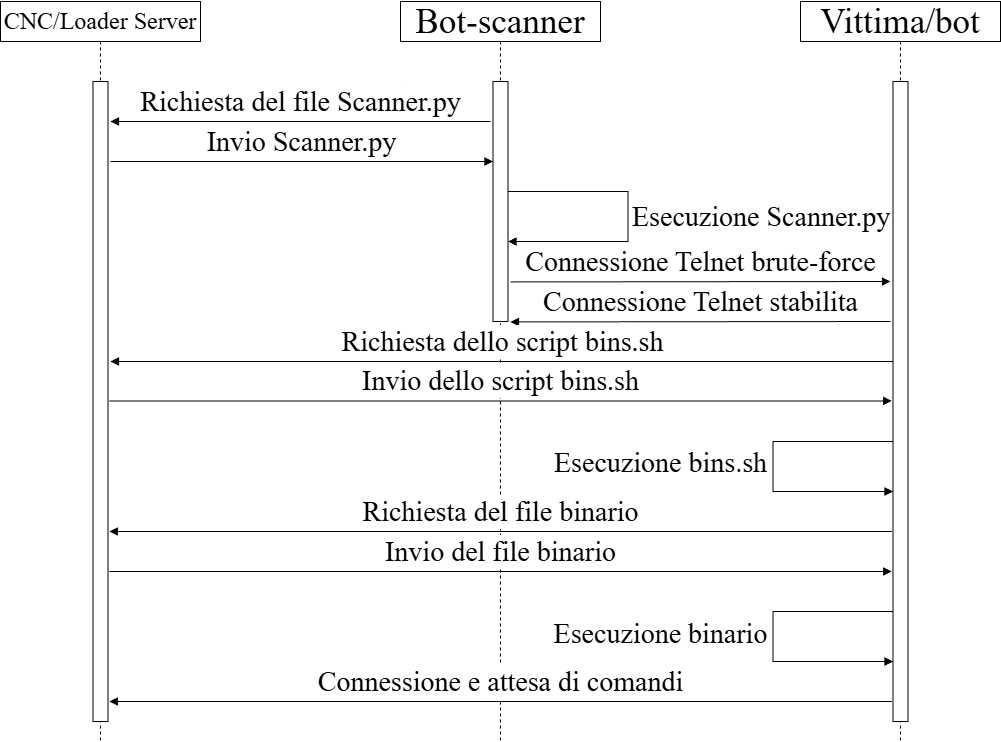
\includegraphics[width=0.75\linewidth]{tesi_stile/img/diagramma_UML_infezione.drawio.png}
    \caption{Sequenza delle operazioni durante la fase di infezione.}
    \label{diagramma_UML_infezione}
\end{figure}